% !TEX root = ./guide-2e.tex
\usepackage{color}
\usepackage{url}
\usepackage{doi}
\usepackage{lmodern}
\usepackage{amsmath}
\usepackage{mathtools}
\usepackage{amsthm}
\usepackage{amssymb}
\usepackage{booktabs}
\usepackage[dvipdfmx]{graphicx}
\usepackage{listings}
\usepackage{float} 
\usepackage{placeins}
\usepackage[nameinlink]{cleveref}
\usepackage{subcaption}

\usepackage{lipsum}

% ADD THE FOLLOWING COUPLE LINES INTO YOUR PREAMBLE
\let\OLDthebibliography\thebibliography
\renewcommand\thebibliography[1]{
  \OLDthebibliography{#1}
  \setlength{\parskip}{0pt}
  \setlength{\itemsep}{0pt plus 0.3ex}
}

\creflabelformat{section}{#2#1#3節}
\creflabelformat{enumerate}{#2#1#3}
\creflabelformat{figure}{#2#1#3}
\creflabelformat{table}{#2#1#3}
\creflabelformat{equation}{#2(#1#3)}
\crefname{section}{}{}
\crefname{enumerate}{}{}
\crefname{figure}{図}{図}
\crefname{table}{表}{表}
\crefname{equation}{式}{式}

\newcommand{\yj}[1]{{#1}^{(\lambda)}}
\newcommand{\yjj}[1]{{#1}^{(\lambda_j)}}
\newcommand{\yjs}[1]{{#1}^{(\lambda*)}}
\newcommand{\tr}[1]{{#1}^\top}
\newcommand{\yjv}{\xi}
\newcommand{\real}{\mathbb{R}}
\newcommand{\cfsq}{$\text{CF}^2$}

%%
\title{
\jtitle{特徴量連続化によるRisk Terrain Modelingの改良}
\etitle{Risk Terrain Modeling on Continuous Features}
}
%%英文は以下を使用
%\title{Style file for manuscripts of JSAI 20XX}

\jaddress{氏名,所属,住所,電話番号,Fax番号,電子メールアドレスなど}

\author{%
\jname{橋本 響}
\ename{Kyo Hashimoto}
\and
\jname{木脇 太一}
\ename{Taichi Kiwaki}
% \and
% \jname{高知大学 理工学部 情報科学科}
% \ename{Department of Information Science, Faculty of Science and Technology, Kochi University}
}

\affiliate{
\jname{高知大学 理工学部 情報科学科}
\ename{Department of Information Science, Faculty of Science and Technology, Kochi University}
% \and
% \jname{\second{}所属和文2}
% \ename{Affiliation \#2 in English}
%\and
%\third{}Affiliation \#3 in English%%英文は左を使用
}

%%
%\Vol{28}        %% <-- 28th(変更しないでください)
%\session{0A0-00}%% <-- 講演ID(必須)

\begin{abstract}
Risk Terrain Modeling(RTM)は,廃屋や廃棄車両などの位置情報から犯罪発生リスクを算出する手法である.
しかし高い空間相関をもつRTMの予測は実際の犯罪発生の特性とは乖離しており,不十分な予測精度として現れていた.
この問題は,特徴量離散化によるモデルの未学習に起因する.
そこで本研究ではRTMの特徴量として連続量の利用を提案した.
この改善に加えて過去の犯罪発生に関する特徴量の追加により,犯罪予測において一般的なPAIの意味で従来手法を24.5\%改善した.
またROC-AUCに関しても統計的に有意な改善が実現された.
\end{abstract}


%\setcounter{page}{1}
\def\Style{``jsaiac.sty''}
\def\BibTeX{{\rm B\kern-.05em{\sc i\kern-.025em b}\kern-.08em%
 T\kern-.1667em\lower.7ex\hbox{E}\kern-.125emX}}
\def\JBibTeX{\leavevmode\lower .6ex\hbox{J}\kern-0.15em\BibTeX}
\def\LaTeXe{\LaTeX\kern.15em2$_{\textstyle\varepsilon}$}

\begin{document}
\maketitle

\section{はじめに}
%----------------------------------------------------------------------------
%\subsection{背景}
%------------------------------------
犯罪の防止は古今を問わず重要な社会課題である.
近年では地理情報システムの発展に伴い,
犯罪が発生した時間・場所などの各種データが蓄積されている\cite{ChicagoDataPortal}.
それらに基づく犯罪予測は,新たな政策提案・警察活動の指針を与えるものとして国際的に期待されている\cite{犯罪予測}.

その代表的手法であるRisk Terrain Modeling(RTM)\cite{caplan2015risk}は,
廃屋や廃棄車両,差し押さえ物件などの位置情報(以下,地理的リスク要因)から作成した特徴量から,
近い将来における犯罪発生リスクを算出・視覚化する手法として広く利用されている\cite{地理的犯罪予測研究の潮流}.
一般的にRTMでは,地理的特徴量は前処理を経て離散的なカテゴリデータへ変換され,線型モデルへ入力される\cite{犯罪予測, caplan2015risk}.
政策立案者や治安維持機関は,RTMにより高リスクエリアを特定し,防犯資源の効率的な配分に役立てる事ができる\cite{犯罪予測}.

%------------------------------------
%\subsection{研究目的}
%\subsection{従来手法の課題}\label{conv_limit:sec}
%------------------------------------
%基盤となる統計モデルは主に線形モデルとして構築されてきた.
しかしRTMにより算出された犯罪リスク値は,実際のデータの特性と乖離した,異常に高い空間相関を持つ.
この特異な振る舞いは不十分な予測精度として現れていた.
この問題点は,特徴量の離散化の結果として予測変数に含まれる情報が制限され,結果としてモデルが未学習することに起因していた.
そこで本研究では離散化を省き,連続的特徴量に対するRTMを提案する.
この改善から情報の損失を抑え,実際の犯罪分布により近しい,RTMによるリスク予測を実現した.
%また定量的な評価としては,犯罪予測の文脈で広く利用されるされる. 
更に地理的リスク要因と並列に犯罪発生情報を予測変数として導入することで,更なる予測精度を向上を実現した.

\section{関連研究}
\label{chapter_2}
%----------------------------------------------------------------------------
\subsection{RTMの実装}
\label{conv_imp:sec}
%------------------------------------
RTM\cite{caplan2015risk}は,
対象地域を特定幅のグリッドで小区画(以下,グリッドセル)へ分割し,各グリッドセルで犯罪発生リスクを予測する.
まず応答変数は,各グリッドセルでの特定種類(e.g., 強盗)の犯罪発生件数である.
予測変数は,地理的リスク要因から生成した離散的特徴量であり,
対象グリッドセル付近におけるリスク要因の空間分布を反映する,以下の2種の特徴量から構成される.

まず一つ目の特徴量はグリッドセル中心に最も近接する地理的リスク要因との距離に関する特徴量である.
具体的には特定のスケールパラメータを用いて距離を2水準(0:スケールパラメータ以上,1:スケールパラメータ未満)へ離散化する.
%
二つ目の特徴量は,地理的リスク要因に対するカーネル密度推定から構成される.
まず各地理的要因について特定のスケールパラメータでカーネル密度推定を実行する\cite{bishop}.
そしてグリッドセル中心における確率密度推定値を2水準(0:平均+2標準偏差未満,1:平均+2標準偏差以上)に離散化する.

これらの方法におけるスケールパラメータはRTMのハイパーパラメータとなる.
これらの適切な設定により,グリッドセル付近における地理的リスク要因の空間分布モデルの空間解像度を調節することが出来る.
またこれらのハイパーパラメータは複数の値を設定し,それぞれで独立に特徴量を構成して,モデルへ並列に組み込むこともできる.

これらの応答変数と予測変数に対して,ポアソン回帰\cite{poisson}か負の二項回帰\cite{Hilbe_2011}を実行する.
更にステップワイズ法\cite{islp}によるBayesian information criteria最小化を通じて変数選択を行い,重要なリスク要因を判定する.
学習後のモデル予測値は犯罪発生リスクとして利用し,それを地図上へヒートマップとして表示したものがリスクマップである.

% % ポアソン回帰 (Poisson Regression)
% \begin{align}\label{poisson}
%    Y_i \sim \text{Poisson}(\lambda_i) \text{,}
%    \log(\lambda_i) = X_i \beta 
%  \end{align}
 
%  % 負の二項回帰 (Negative Binomial Regression)
%  \begin{align}\label{negative binominal}
%    Y_i \sim \text{NB}(\mu_i, \theta) \text{,}
%    \log(\mu_i) = X_i \beta 
%  \end{align}
 
%  この手法では,地理的リスク要因による特徴量を離散的なカテゴリデータとして表現している.
%  例えば,各グリッドセルが特定の地理的リスク要因から,
%  一定距離内に存在するか否かを$0$または$1$で表す.

%------------------------------------
\subsection{予測精度向上への取り組み}
%------------------------------------
% 大山ら\cite{大山智也2020短期的}は,最新の犯罪発生に伴う短期的なリスクと,
% RTMの予測因子では捉えきれない長期的なリスクを組み合わせることで,RTMを発展させた.
% この改善により,既存のRTMを上回る予測精度と安定性を得た.
% このことは,地理的リスク要因以外の環境要因や再犯リスクを考慮することで,
% どの時期でも安定した予測が可能になることを示唆している.
大山\cite{大山智也2020日本}は,RTMに対して犯罪発生情報を組み合わせることで,
中長期的な潜在リスクに加えて,短期的な顕在リスクも算出するモデルを構築した.
この改善により,的中率においてはRTMをを上回る予測精度を得たが,predictive accuracy index(PAI)はRTMを下回る結果となった.

\begin{table}[t]
  \centering
  \caption{2011年から2014年のデータ}
  \label{tab:2011-2014-data}
  \begin{tabular}{lrrrr}
  \toprule
  カテゴリ & 2011 & 2012 & 2013 & 2014 \\
  \midrule
  強盗 & 26577 & 22783 & 17854 & 14490 \\
  \midrule
  廃墟 & 15365 & 11971 & 8363 & 5446 \\
  放置車両 & 19907 & 17390 & 16077 & 20358 \\
  路地灯消灯 & 46697 & 19944 & 15177 & 21684 \\
  街灯消灯 & 33895 & 30893 & 22650 & 64857 \\
  学校 & 674 & 681 & 672 & 680 \\
  差し押さえ物件 & 16680 & 16120 & 11131 & 7511 \\
  落書き除去 & 136873 & 109908 & 137058 & 124721 \\
  不衛生な場所 & 17888 & 19088 & 18029 & 18997 \\
  \midrule
  暴行 & 60306 & 58998 & 53887 & 49230 \\
  器物損壊 & 37234 & 35771 & 30779 & 27637 \\
  窃盗 & 74770 & 75170 & 71270 & 61127 \\
  性的暴行 & 1402 & 1347 & 1197 & 1216 \\
  売春 & 2424 & 2200 & 1652 & 1608 \\
  賭博 & 736 & 724 & 596 & 393 \\
  酒類法違反 & 619 & 573 & 464 & 394 \\
  武器違反 & 3879 & 3904 & 3240 & 3099 \\
  誘拐 & 266 & 234 & 242 & 217 \\
  公務執行妨害 & 1041 & 1227 & 1277 & 1393 \\
  傷害 & 20343 & 19848 & 17920 & 16830 \\
  殺人 & 437 & 515 & 431 & 428 \\
  性犯罪 & 1053 & 1035 & 1004 & 909 \\
  詐欺行為 & 12329 & 13239 & 13215 & 14788 \\
  自動車盗難 & 19353 & 16450 & 12552 & 9846 \\
  薬物犯罪 & 38527 & 35417 & 34057 & 28836 \\
  放火 & 504 & 469 & 363 & 394 \\
  脅迫 & 171 & 156 & 133 & 114 \\
  児童関連犯罪 & 2281 & 2190 & 2319 & 2304 \\
  不法侵入 & 8634 & 8197 & 8122 & 7500 \\
  ストーカー行為 & 181 & 206 & 153 & 140 \\
  治安妨害 & 3089 & 3001 & 3131 & 2896 \\
  その他の犯罪 & 20134 & 17471 & 17979 & 16902 \\
  \bottomrule
  \end{tabular}
  \end{table}

%----------------------------------------------------------------------------
\section{提案手法}
\label{chapter_3}
%----------------------------------------------------------------------------
RTMの特徴量構成法は離散化により予測変数の情報が十分にモデルへ伝わらず,結果としてモデルが未学習となる可能性がある.
また\cref{conv_imp:sec}で述べた様に,\cite{caplan2015risk}のRTM実装は古典的なステップワイズ法\cite{islp}による変数選択に依存するが,同等の効果はより効率的なLasso回帰\cite{Lasso}でも実現できる.これら点から,本研究では以下へ取り組む:
\begin{enumerate}
  \item 未学習防止のための連続型特徴量導入,
  \item Power transformとLasso回帰によるモデル構成.
\end{enumerate}
%この改善によるモデルを連続RTMとする(単にRTMと書いた時は\citet{caplan2015risk}による元々の実装を指すとする).
% note:こう書いてしまうと実験セクションでのベースラインにCaplanのRTMを使う必要が出て来てしまう.

\begin{figure}
  \centering 
  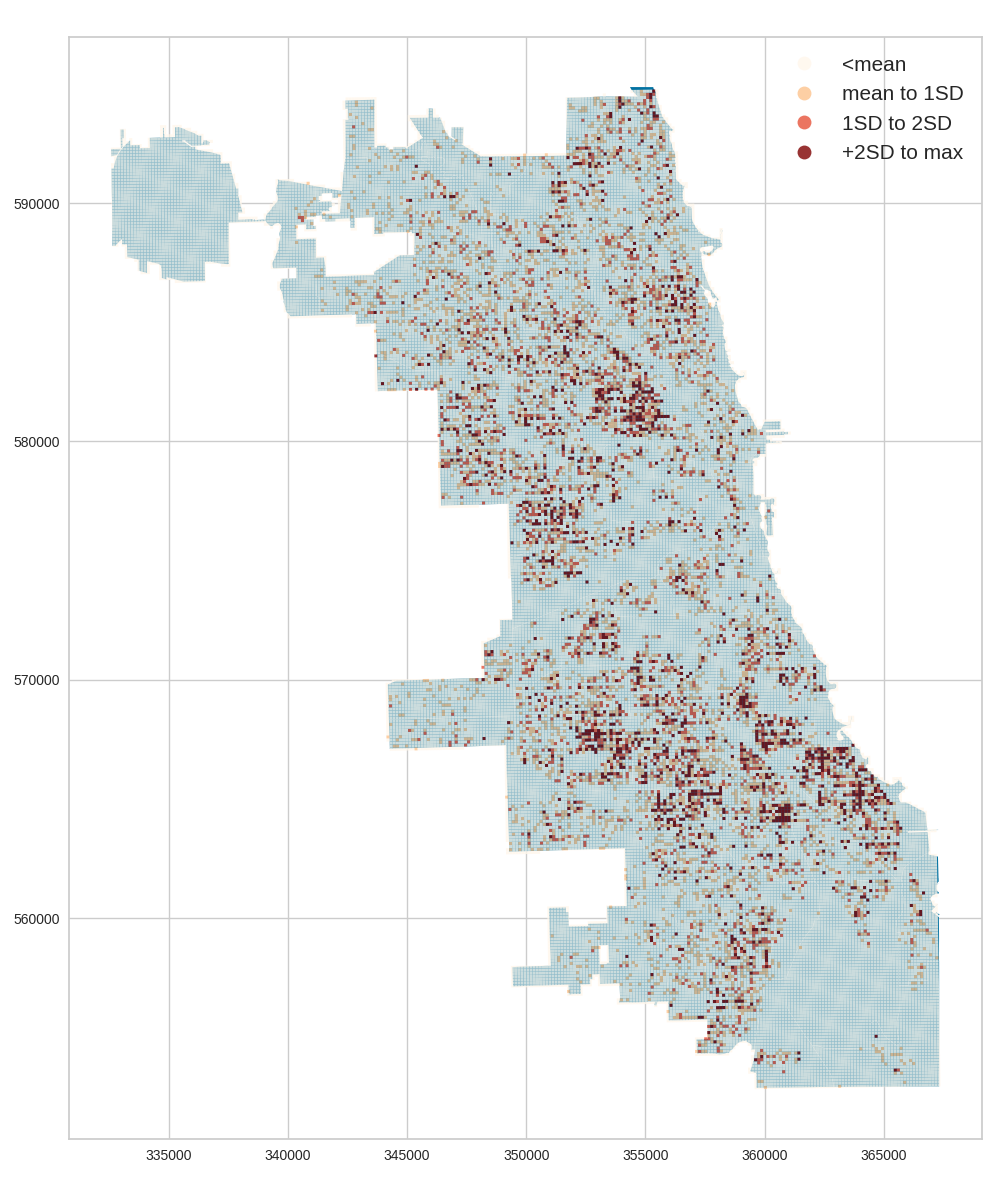
\includegraphics[scale=0.25]{./figures/actual_riskmap.png}
  \caption{真のリスクマップ}
  \label{fig:non-crime-timeseries-actual-risk}
\end{figure}


\begin{figure*}[t]
  \centering 
  \begin{subfigure}{0.3\textwidth}
    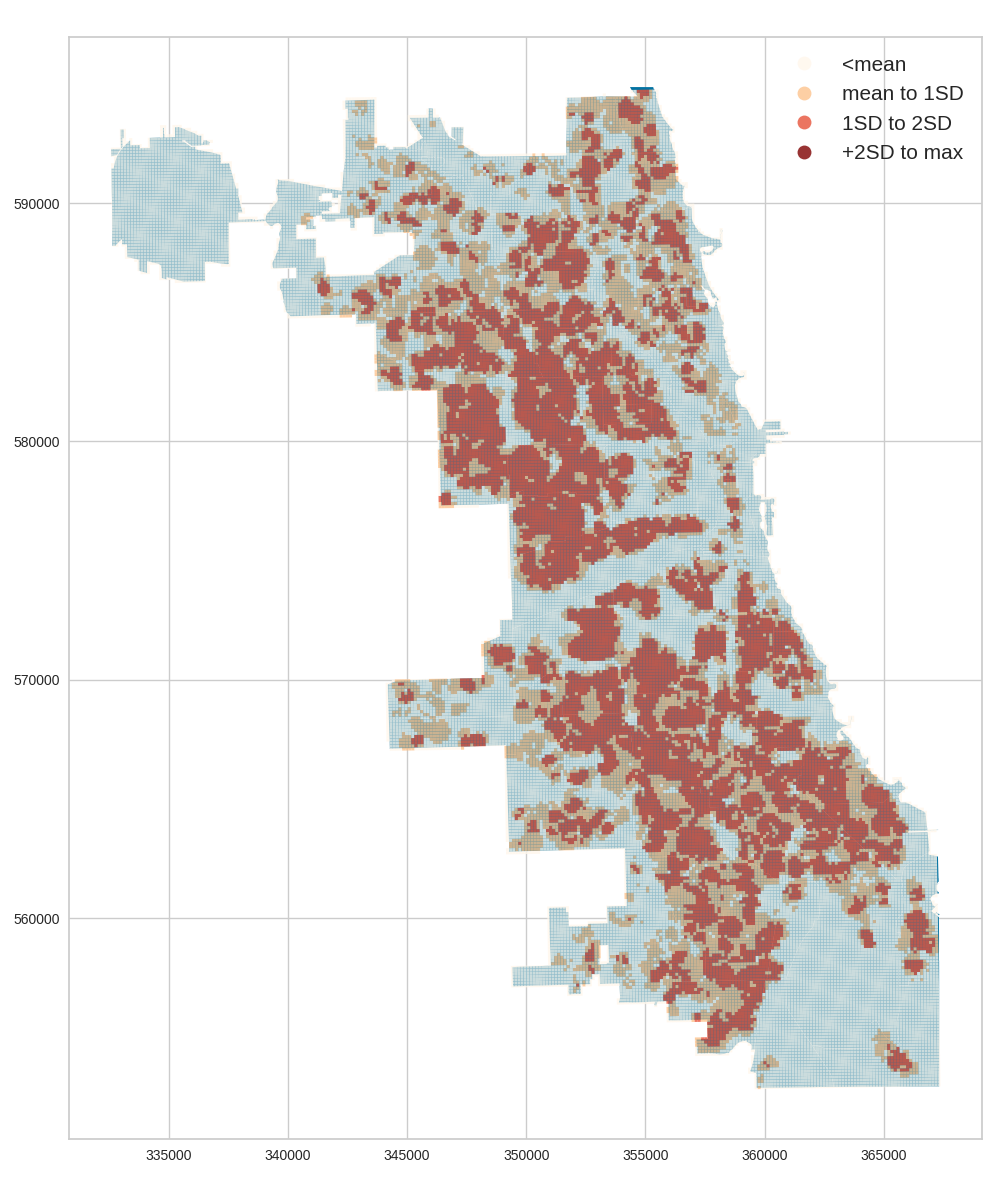
\includegraphics[scale=0.25]{./figures/DF_riskmap.png}
    \caption{DF}
    \label{fig:non-crime-timeseries-df-risk}
  \end{subfigure}
  \begin{subfigure}{0.3\textwidth}
    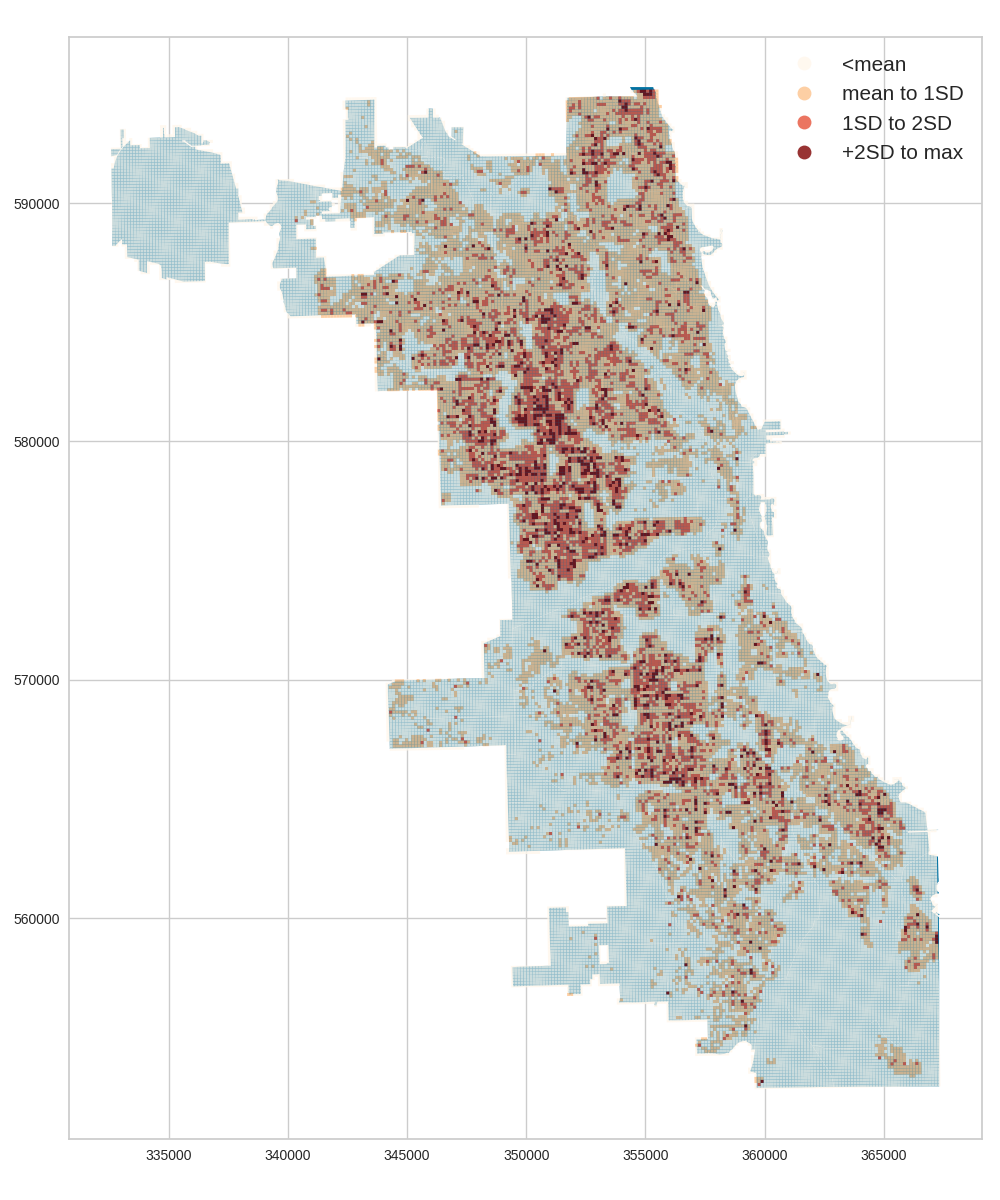
\includegraphics[scale=0.25]{./figures/CF_riskmap.png}
    \caption{CF}
    \label{fig:non-crime-timeseries-cf-risk}
  \end{subfigure}
  \begin{subfigure}{0.3\textwidth}
    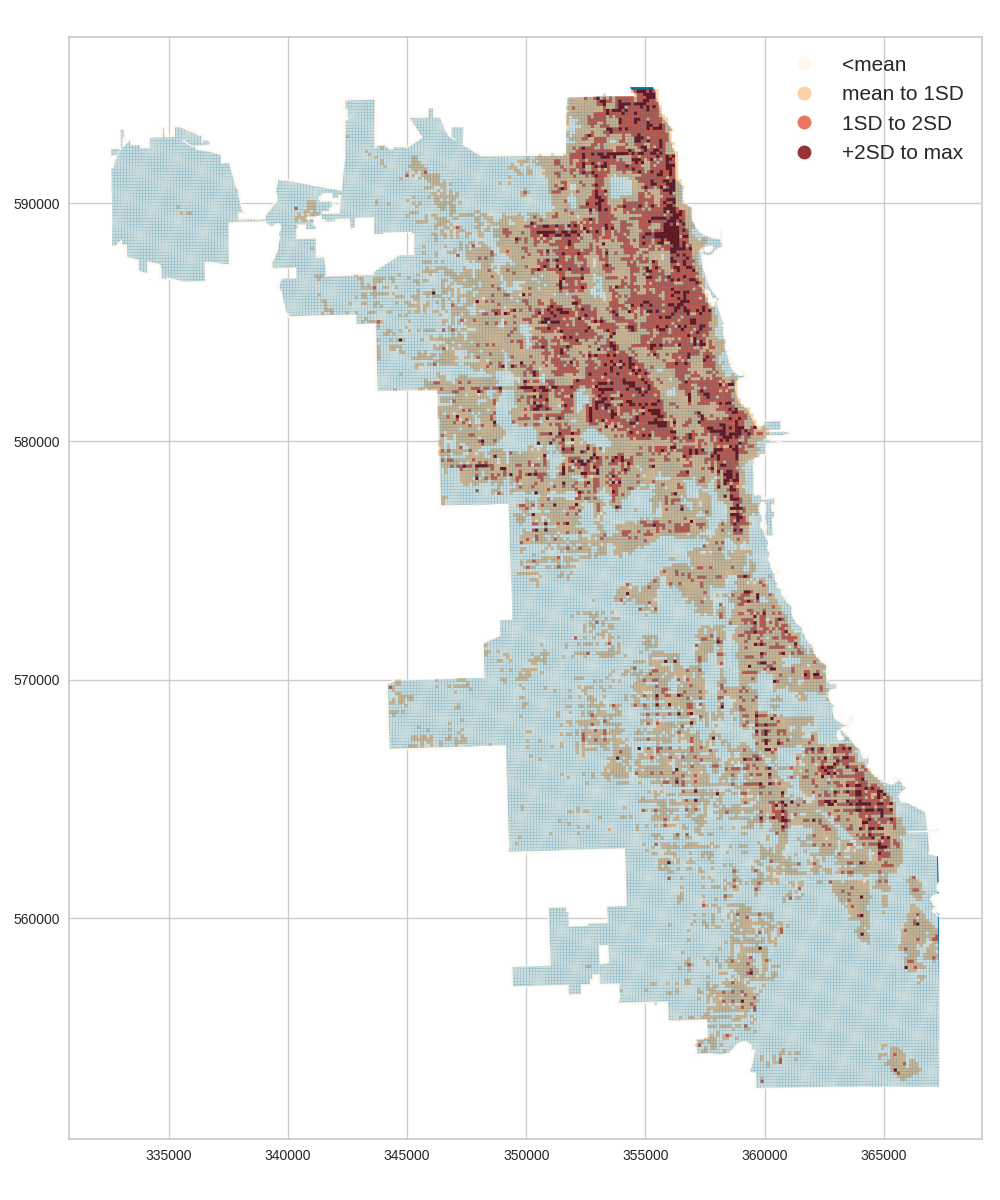
\includegraphics[scale=0.25]{./figures/CI_riskmap.png}
    \caption{\cfsq}
    \label{fig:non-crime-timeseries-ci-risk}
  \end{subfigure}
  \label{fig:non-crime-timeseries-risks}
  \caption{各手法によるリスクマップの比較}
\end{figure*}


%------------------------------------
\subsection{連続型特徴量}
%------------------------------------
従来手法\cite{caplan2015risk}では,グリッドセル中心から地理的リスク要因への最短距離,およびカーネル密度推定値を離散化するが,
提案手法ではその工程を省き,元々の連続値をそのまま特徴量とする.この特徴量構成法をcontinuous features(CF)と呼ぶ.

% %------------------------------------
% \subsection{犯罪特徴量を追加した連続化(Continuous  Features Including Crime Features, CI)}
% %------------------------------------
% 従来手法\cite{caplan2015risk}では,応答変数以外の犯罪発生情報を予測に用いていなかった.
% 犯罪発生情報を予測に取り入れる手法は先行研究\cite{大山智也2020日本}でも提案されているが,
% 予測精度が向上したとはいえない.
% そこでCIではCFの発展として,応答変数以外の犯罪発生情報を連続型特徴量としてRTMの予測変数とする.
%------------------------------------
\subsection{Lasso回帰によるRTMの実装}
%------------------------------------
まずLasso回帰を実行するにあたって,応答変数の分布が正規分布から大きく乖離している場合には適切な学習が難しくなると知られている\cite{islp, esl}.一方で,犯罪の発生分布は多くの地域で治安が良い反面で,一部の犯罪多発地域も存在する.つまり犯罪の発生分布は大きな歪みと裾の重さを持ち,従って正規分布とは大きく乖離したものとなる.
%

この問題へ対処するため本研究では前処理として,応答変数と予測変数をYeo-Johnson変換\cite{yeo}する:
\begin{equation*}\label{yeo:eq}
  \yj{\yjv} =
   \begin{cases} 
   \frac{(\yjv+1)^\lambda - 1}{\lambda}, & \text{if } \lambda \neq 0, \yjv \geq 0,  \\ 
   \log(\yjv+1), & \text{if } \lambda = 0, \yjv \geq 0,   \\ 
   \frac{-(-\yjv+1)^{2-\lambda} + 1}{2-\lambda}, & \text{if } \lambda \neq 2, \yjv < 0,  \\ 
   -\log(-\yjv+1) & \text{if } \lambda = 2, \yjv. < 0
   \end{cases}
\end{equation*}
ここで$\yjv$は変換前の値,$\yj{\yjv}$は変換後の値であり,$\lambda$はデータから推定される変換パラメータである.
またYeo-Johnson変換の逆変換は以下となる:
\begin{equation*}\label{yeo_inv:eq}
  \yjv =
  \begin{cases} 
    (\lambda\yj{\yjv}+1)^{\frac{1}{\lambda}}-1, & \text{if } \lambda \neq 0, \yjv \geq 0,  \\ 
  \exp(\yj{\yjv})-1, & \text{if } \lambda = 0, \yjv \geq 0,   \\ 
  1-(1-(2-\lambda)\yj{\yjv})^{\frac{1}{2-\lambda}}, & \text{if } \lambda \neq 2, \yjv < 0,  \\ 
  1-\exp(-\yj{\yjv}), & \text{if } \lambda = 2,  \yjv < 0.
  \end{cases}
\end{equation*}

$i$番目のグリッドセルにおける応答変数を$y_i$,またその$j$番目の地理的リスク要因に関する特徴量を$x_{ij}$とする($i=1,\cdots, n,\quad j=0,\cdots, d$.ただし$j=0$はバイアス項に対応).これらのYeo-Johnson変換結果を$\yj{y_i}, \yjj{x_{ij}}$とすれば,Lasso回帰は以下の目的関数の最小化として実現される\cite{Lasso}:
\begin{align} \label{lasso_loss:eq}
  L_\mathrm{lasso}(w) := \frac{1}{n}\sum_{i=1}^n\left\|
    \yj{y}_i-\tr{w}{\yjs{x_i}}
    \right\|^2 + \nu\sum_{j=1}^{d}|w_j|. 
\end{align}
ここで$\yjs{x}$は$\yjj{x_j}$を集めたベクトル,$w=\tr{(w_0, \cdots, w_d)}\in\real^{d+1}$は係数ベクトル,$\nu>0$は正則化の強度を制御するハイパーパラメータである.\cref{lasso_loss:eq}の最小化で得られる係数ベクトルを$\hat w$とする.
Lassoの利用により,予測への寄与の小さい変数の重み$\hat w_j$が自動的に$0$となり,変数選択が実現される\cite{Lasso, islp, esl}.

新たに追加された区画における予測変数を$x=\tr{(1, x_1, \cdots, x_d)}$,そのYeo-Johnson変換を$\yjs{x}$とすれば,その区画での犯罪リスクは$\hat w$を用いて
\begin{align*}
 {\yj{\hat y}} = \tr{\hat w} \yjs{x}
\end{align*}
と算出できる.ただし$\yj{\hat y}$はYeo-Johnson変換後の値として意味を持つので,直接解釈は出来ない.そのため,リスクマップを構成する際には,$\yj{\hat y}$へYeo-Johnson逆変換を施した$\hat y$を用いる.
%\yj{y}_i

% モデルの出力値に対して,Yeo-Johnson逆変換を行って,
% 予測値の分布を元の犯罪の分布に近づけた.モデルの予測値は連続値であるため,
% 精度評価やリスクマップ表示の際には,予測値をそれぞれを適切な基準で離散化する.
 
以降,本論文におけるRTMの実装は\cite{caplan2015risk}のものでは無く,本節で述べたLassoによるものとする。



%----------------------------------------------------------------------------
\section{実験}
%----------------------------------------------------------------------------

本節では1)\cite{caplan2015risk}に準ずる離散化を伴う特徴量構成法(discrete features,DF),2)提案手法CF,3)CFを基に過去の犯罪発生状況\cite{大山智也2020日本}を追加した特徴量構成法(continuous features $\times$ criminal features, \cfsq)の3種の特徴量構成法を,実データに対する実験を通じて比較する.

%------------------------------------
\subsection{データセット}
本研究では,\cite{caplan2015risk}が提案するRTMと同様に,
アメリカ合衆国のイリノイ州クック郡の郡庁所在地であるシカゴ市を対象領域とする.
応答変数を構成する犯罪発生地点及び,予測変数を構成する地理的リスク要因の位置情報は,
\cite{ChicagoDataPortal}のAPIを用いて緯度経度情報として取得した.

取得したデータ期間は2011年1月1日〜2014年12月31日で,
それぞれの犯罪発生地点と地理的リスク要因の位置情報は,
ともに発生時刻・記録年を基に1年単位で取得した.
表\ref{tab:2011-2014-data}に取得した全データ件数を示す.



%------------------------------------
\subsection{評価指標}\label{sec:criteria}
%------------------------------------
まず性能評価に際してはモデルが予測した犯罪発生リスクを,
高リスク($平均+1標準偏差以上$)と低リスク($平均+1標準偏差未満$)にカテゴリー化する.
これにより分類問題として問題を捉え直し,評価を行う.

評価指標としては,犯罪予測の文脈で一般的な
的中率\cite{joshi2020considerationsdevelopingpredictivemodels}ならびに
PAI\cite{chainey2008utility}に加え,分類学習で一般的なarea under the receiver operating characteristic(ROC) curve\cite{islp}を用いた.

的中率とは,予測モデルが「高リスク」と特定したエリアの中で、実際に犯罪が発生した割合である:
\begin{equation}\label{hitrate}
  的中率=\frac{高リスク判定エリア内の犯罪数}{全エリアの犯罪数}.
\end{equation}
%(\ref{hitrate})式に的中率の計算式を示す.
しかし高リスク判定エリアにおける犯罪件数のみに依存する的中率は,低リスクエリアを高リスクエリアと誤って識別する偽陽性を評価できない.すなわち的中率を最大とするモデルは,単に高リスク判定を出し易くする一方で,その大多数が誤報である可能性が残る.
%
そのため本研究では,的中率に加えてPAI\cite{chainey2008utility}も評価に用いる.
PAIは,高リスクエリア内で発生した犯罪の割合を、そのエリアの全体に占める面積割合で除した値である.
\begin{equation}\label{pai}
  \mathrm{PAI}=\frac{的中率}{\frac{高リスクエリア面積}{全エリア面積}}.
\end{equation}
PAIでは高リスクエリア面積割合を分母に置くことで,的中率が評価する真陽性に加えて偽陽性の影響も加味したものである.

偽陽性と真陽性のバランスを評価する指標は機械学習の文脈でも多く知られるが,その代表例としてarea under the ROC curve(ROC-AUC)がある\cite{islp}.RTMによる犯罪リスク値$\hat y$を予測スコアとすれば,ROC-AUCを以てしてもRTMの性能評価が実施できるため,本研究では評価に取り入れる.

\begin{figure}
  \centering 
  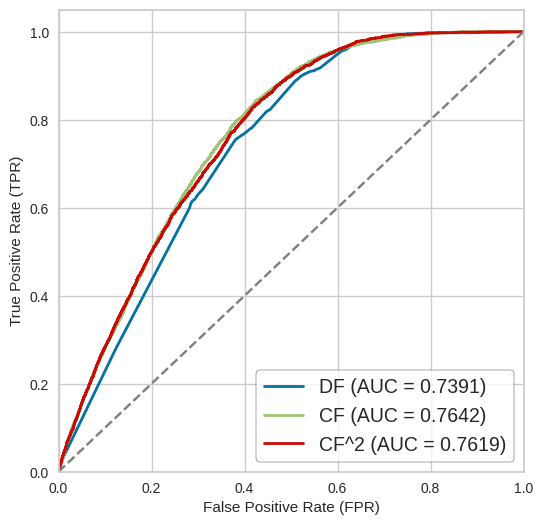
\includegraphics[scale=0.25]{./figures/roc.png}
  \caption{各手法のROC曲線}
  \label{fig:roc}
\end{figure}
\begin{table}[htbp]
  \centering
  \caption{各モデル間の精度比較}
  \begin{tabular}{l|r||r|r}
  \hline

  モデル & DF & CF & \cfsq \\  \hline\hline
  的中率 & \bf{57.2} & 30.2 & 31.3  \\ 
  PAI & 1.84 & 2.18 & \bf{2.29} \\ 
  AUC & 0.74 & \bf{0.76} & \bf{0.76} \\ \hline
  \end{tabular}
  \label{tb:fig:non-crime-timeseries-index}
\end{table}



\subsection{実験条件}
%------------------------------------
%\subsection{RTMの実装条件}
%------------------------------------
取得したデータは,地理的座標系に基づいており,緯度経度情報として提供されているが,
本研究では距離計算や空間分析を正確に行うため,PythonのGeoPandasライブラリー\cite{geopandas}を使用し,
メートル単位での解析が可能な平面直角座標系(EPSG:26971)に変換した.
また,データ品質を保証するため,明らかに誤った位置情報(NaN,0,etc.)と
シカゴ市領域外の位置情報は事前に除外した.

また対象地域に設定したグリッドは130m$\times$130mである.
なお,特徴量構成に関わるスケールパラメータは271m, 591m, 779m, 1003mであり,これらで構成した特徴量はモデルへ並列に入力した.
これらのスケールパラメータの値はシカゴ市の2,4,6,8ブロックに相当する.

応答変数は,各グリッドセル内で発生した強盗犯罪件数とした.
予測変数として用いた地理的リスク要因は,\cref{tab:2011-2014-data}に示す通り
廃屋,放置車両,路地灯消灯,街灯消灯,学校,差し押さえ物件,落書き除去,不衛生な場所
の8つである.

前処理におけるYeo-Johnson変換・逆変換,そしてLasso回帰には,sklearn\cite{scikit-learn}の実装を用いた.
なおLasso回帰による変数選択を適切に実行するため,前処理として予測変数の標準化も実施した.

%------------------------------------
学習データとテストデータの分割は以下の通りである.まず季節変動を除くため,分割の単位は年単位とした.
また予測変数の構成にあたってはデータリークを防ぐため,ある年の応答変数の予測には前年の予測変数を利用した(2010年の予測変数は取得できなかったので,2011年の応答変数は利用していない).
これを踏まえて本研究では,2012年および2013年の応答変数とそれぞれ対応する予測変数を学習データとし,2014年の応答変数と2013年の予測変数をテストデータとして設定した.探索の必要があるハイパーパラメータはLasso回帰の正則化パラメータ$\nu$であるが,この最適化は学習データに対する20分割交差検証で行った.

%------------------------------------
\subsection{結果}
テストデータから算出した2014年の強盗犯罪に関わるリスクマップ(以下,真のリスクマップ)を\cref{fig:non-crime-timeseries-actual-risk}に示す.
またDF, CF, \cfsq の各手法によるリスクマップを\cref{fig:non-crime-timeseries-risks}に示す.
真のリスクマップと比べて,DFによるリスクマップは高い空間相関を持つ.
一方,CFと\cfsq によるリスクマップは空間相関が削減されていることが観察できる.
これはDFでは離散化に起因した未学習が起きていることに対して,CF・\cfsq ではこの問題が改善されていると理解できる.

各手法による予測の定量的な評価結果を\cref{tb:fig:non-crime-timeseries-index}にまとめる.
的中率が最も高いのはDFであるが,\cref{sec:criteria}で述べた通り的中率では偽陽性を評価できないため,PAIとAUCに注目する.
PAIは,CFにより大きく改善し,\cfsq では更なる改善が確認できた.
次にAUCは,CF・\cfsq で同等の改善が確認できた.
またDFと\cfsq のAUC値の有意差を評価するためにDeLong検定\cite{DeLong}を実施した結果,
$p<0.001$となり,提案手法によるROC-AUCの改善が統計的に有意であると確認できた.
同様の傾向は\cref{fig:roc}に示すROC曲線からも観察できる.


%----------------------------------------------------------------------------
\section{おわりに}
%----------------------------------------------------------------------------
本研究で提案した連続特徴量はリスクマップの空間相関削減に寄与し,さらに従来手法を上回る予測性能を実現した.
またPAIに限っては,連続特徴量の利用に加えて,過去の犯罪発生情報の組み込みでも改善を確認した.
また加えてLasso回帰を中核とするRTMの実装法も提案した.
%犯罪予測の文脈では,特徴量構成法の改善は一般的ではないが,RTMにおいては予測精度の向上と空間相関の削減につながることが確認できた.
%犯罪発生情報をRTMに取り入れることは,RTMを導入するモチベーションから離れてしまうが,犯罪予測モデルとしては,他犯罪種の発生情報を予測に取り入れる試みが既存のRTMを上回る予測精度を得ることが確認できた.

%また従来手法によるRTMのアルゴリズムを簡略化して再実装することにより,製品版RTMを利用するだけでは至らなかった改善を実施することができた.

% \begin{thebibliography}{}

  \bibitem[Bishop 07]{bishop}
  Bishop,~C.~M.: {\em Pattern Recognition and Machine Learning (Information Science and Statistics)}, Springer, 1 edition (2007)
  
  \bibitem[Caplan 15]{caplan2015risk}
  Caplan,~J.~M.et al.: Risk terrain modeling for spatial risk assessment, {\em Cityscape}, Vol.~17, No.~1, pp. 7--16 (2015)
  
  \bibitem[CDPH 24]{ChicagoDataPortal}
  Chicago Department of Public Health. (2024), \url{https://data.cityofchicago.org/}
  
  \bibitem[Chainey 08]{chainey2008utility}
  Chainey,~S. et al.: The utility of hotspot mapping for predicting spatial patterns of crime, {\em Security journal}, Vol.~21, pp. 4--28 (2008)
  
  \bibitem[DeLong 88]{DeLong}
  DeLong,~E.~R., et al.: Comparing the Areas under Two or More Correlated Receiver Operating Characteristic Curves: A Nonparametric Approach, {\em Biometrics}, Vol.~44, No.~3, pp. 837--845 (1988)
  
  \bibitem[Hastie 01]{esl}
  Hastie,~T., et al.: {\em The Elements of Statistical Learning}, Springer Series in Statistics, Springer New York Inc., New York, NY, USA (2001)
  
  \bibitem[Hilbe 11]{Hilbe_2011}
  Hilbe,~J.~M.: {\em Negative Binomial Regression}, Cambridge University Press, 2 edition (2011)

  \bibitem[Yeo 00]{yeo}
  I. Yeo , R. Johnson: A new family of power transformations to improve normality or symmetry {\em Biometrika}, vol. 87, pp. 954--959, (2000)

  \bibitem[James 23]{islp}
  James,~G., et al.: {\em An Introduction to Statistical Learning with Applications in Python}, Springer Texts in Statistics, Springer, Cham (2023)
  
  \bibitem[Jordahl 20]{geopandas}
  Jordahl,~K., et al.: geopandas/geopandas: v0.8.1 (2020)
  
  \bibitem[Joshi 20]{joshi2020considerationsdevelopingpredictivemodels}
  Joshi,~C. et al.: Considerations for developing predictive models of crime and new methods for measuring their accuracy (2020)
  
  \bibitem[Nelder 72]{poisson}
  Nelder,~J.~A., Wedderburn,~R.~W.~M.: Generalized Linear Models, {\em Journal of the Royal Statistical Society. Series A (General)}, Vol. 135, No.~3, pp. 370--384 (1972)
  
  \bibitem[Pedregosa 11]{scikit-learn}
  Pedregosa,~F. et al.: Scikit-learn: Machine Learning in {P}ython, {\em Journal of Machine Learning Research}, Vol.~12, pp. 2825--2830 (2011)
  
  \bibitem[Tibshirani 96]{Lasso}
  Tibshirani,~R.: Regression shrinkage and selection via the lasso, {\em Journal of the Royal Statistical Society Series B: Statistical Methodology}, Vol.~58, No.~1, pp. 267--288 (1996)
  
  \bibitem[守山 22]{犯罪予測}
  守山正:犯罪予測 : AIによる分析, 成文堂 (2022)
  
  \bibitem[大山 17]{地理的犯罪予測研究の潮流}
  大山智也 et al.:地理的犯罪予測研究の潮流, GIS-理論と応用, Vol.~25, No.~1, pp. 33--43 (2017)
  
  \bibitem[大山 20]{大山智也2020日本}
  大山智也:日本における地理的犯罪予測手法の開発に関する研究 (2020)
  
  \end{thebibliography}
  

\bibliography{main}
\bibliographystyle{jsai}

%%
